\section{روش‌های کنترل}
\label{sec:controllers}

در این بخش، روش‌های کنترل پیاده‌سازی‌شده برای پایدارسازی پاندول معکوس با چرخ واکنشی را معرفی می‌کنیم. تمامی کنترلرها یک فرمان \textbf{ولتاژ} $V$ به مدار آرمیچر موتور DC اعمال می‌کنند. ولتاژ خروجی همواره در محدوده مجاز اشباع می‌شود:

\begin{equation}
V_{\text{applied}} = \operatorname{clip}(V,\; -V_{\max},\; V_{\max})
\end{equation}

این محدودیت، رفتار واقعی عملگر الکتریکی را منعکس می‌کند؛ زیرا ولتاژ قابل اعمال به آرمیچر در عمل محدود است.

پیش از معرفی کنترلرها، یادآوری می‌کنیم که بردار حالت سیستم به صورت زیر تعریف شده است:

\begin{equation}
\mathbf{x} = \begin{bmatrix} \theta & \dot{\theta} & \varphi & \dot{\varphi} & i_a \end{bmatrix}^\top
\end{equation}

که در آن $\theta$ زاویه پاندول، $\varphi$ زاویه چرخ واکنشی و $i_a$ جریان آرمیچر است. دینامیک مکانیکی سیستم از ماتریس اینرسی کوپل‌شده $2 \times 2$ و دینامیک الکتریکی از معادله مدار آرمیچر به‌دست می‌آید. کنترلرها مستقیماً گشتاور محاسبه نمی‌کنند؛ بلکه ولتاژ ورودی را مشخص می‌کنند و فیزیک موتور (اتصال مستقیم، $N=1$) به‌صورت داخلی در شبیه‌ساز، ولتاژ را به گشتاور چرخ تبدیل می‌کند.

% ─────────────────────────────────────────────────────────────────────
\subsection{بدون کنترل}

ساده‌ترین حالت ممکن، اعمال ولتاژ صفر است:

\begin{equation}
V = 0
\end{equation}

در این حالت، پاندول تنها تحت اثر گرانش و میرایی حرکت می‌کند و هیچ نیروی اصلاحی اعمال نمی‌شود. از آنجا که نقطه تعادل عمودی پاندول معکوس ناپایدار است، سیستم در این حالت از تعادل خارج شده و سقوط می‌کند. این حالت برای مشاهده پاسخ حلقه‌باز سیستم و مقایسه عملکرد کنترلرها مفید است.

شکل~\ref{fig:open-loop} پاسخ حلقه‌باز پاندول را از زاویه اولیه $\theta_0 = 0.1$ رادیان بدون اعمال هیچ فرمان کنترلی نشان می‌دهد. همان‌طور که انتظار می‌رود، پاندول تحت اثر گشتاور گرانشی از وضعیت عمودی فاصله گرفته و سقوط می‌کند.

\begin{figure}[H]
\centering
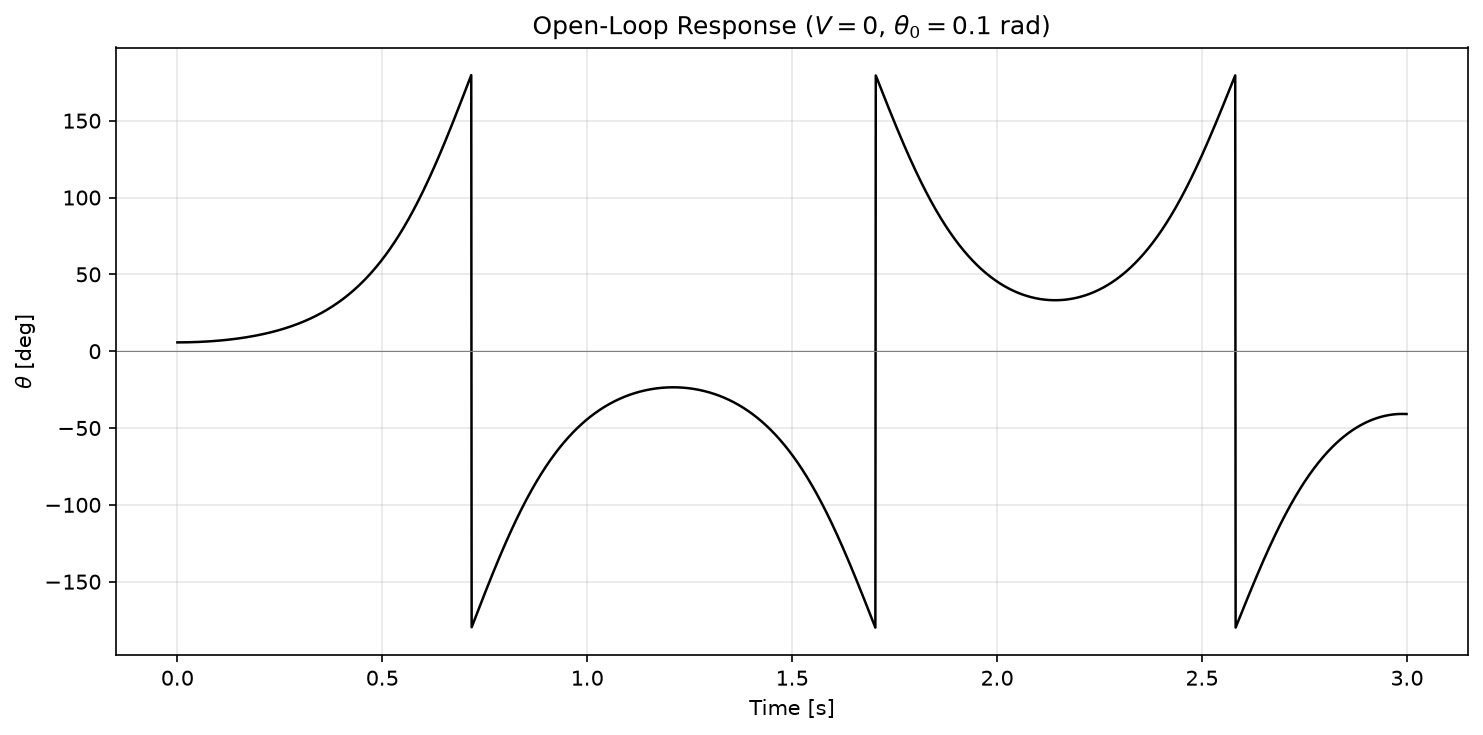
\includegraphics[width=0.85\textwidth]{results/open_loop_response.png}
\caption{پاسخ حلقه‌باز پاندول معکوس بدون کنترل ($\theta_0 = 0.1$ رادیان)}
\label{fig:open-loop}
\end{figure}

% ─────────────────────────────────────────────────────────────────────
\subsection{کنترل دستی}

در حالت کنترل دستی، کاربر یک ولتاژ ثابت $V_{\text{set}}$ را مشخص می‌کند و این ولتاژ پس از اعمال محدودیت اشباع به آرمیچر فرستاده می‌شود:

\begin{equation}
V = \operatorname{clip}(V_{\text{set}},\; -V_{\max},\; V_{\max})
\end{equation}

در این حالت هیچ بازخوردی از وضعیت سیستم وجود ندارد. کاربرد اصلی این حالت، آزمایش‌های حلقه‌باز و شناسایی رفتار سیستم است.

% ─────────────────────────────────────────────────────────────────────
\subsection{کنترلر PID}

\subsubsection{قانون کنترل}

کنترلر PID زاویه پاندول $\theta$ را حول نقطه تعادل عمودی ($\theta = 0$) تنظیم می‌کند. سیگنال کنترلی به صورت زیر محاسبه می‌شود:

\begin{equation}
V = K_p\, \theta + K_i \int_0^t \theta(\tau)\, d\tau + K_d\, \dot{\theta}
\end{equation}

هر یک از بهره‌ها نقش مشخصی در رفتار سیستم دارند:

\begin{itemize}[itemsep=2pt]
    \item $K_p$ (بهره تناسبی): اصلاح متناسب با خطای زاویه. افزایش این بهره سرعت پاسخ را بالا می‌برد، اما ممکن است باعث افزایش نوسان شود.
    \item $K_i$ (بهره انتگرالی): حذف خطای ماندگار. این جمله انحراف ثابت از نقطه تعادل را در طول زمان جبران می‌کند.
    \item $K_d$ (بهره مشتقی): میرایی متناسب با سرعت زاویه‌ای. این جمله نوسانات را کاهش می‌دهد و پایداری را بهبود می‌بخشد.
\end{itemize}

قرارداد علامت به این صورت است که زاویه مثبت $\theta$ نیازمند ولتاژ اصلاحی مثبت است.

\subsubsection{جلوگیری از اشباع انتگرال}

یکی از مشکلات رایج کنترلرهای PID در حضور محدودیت عملگر، پدیده باد کردن انتگرال (Integral Windup) است. هنگامی که خروجی کنترلر در اشباع قرار دارد، جمله انتگرالی به تجمع ادامه می‌دهد و پس از خروج از اشباع، باعث پاسخ بیش‌ازحد و تأخیر در بازیابی می‌شود.

برای مقابله با این پدیده، از روش توقف شرطی (Clamping) استفاده می‌کنیم. در هر گام زمانی با فاصله $\Delta t$، ابتدا خروجی آزمایشی محاسبه می‌شود:

\begin{equation}
u_{\text{trial}} = K_p\,\theta + K_i\,I + K_d\,\dot{\theta}
\end{equation}

که در آن $I$ مقدار تجمعی انتگرال است. قانون به‌روزرسانی انتگرال به صورت زیر است:

\begin{itemize}[itemsep=2pt]
    \item اگر $|u_{\text{trial}}| < V_{\max}$، انتگرال به‌صورت عادی به‌روز می‌شود:
    \begin{equation}
    I \leftarrow I + \theta\,\Delta t
    \end{equation}
    \item اگر $|u_{\text{trial}}| \ge V_{\max}$، انتگرال تنها در صورتی به‌روز می‌شود که تجمع آن در جهت کاهش اشباع باشد:
    \begin{equation}
    I \leftarrow I + \theta\,\Delta t \quad \text{if} \quad (u_{\text{trial}} > 0 \;\wedge\; \theta < 0) \;\;\vee\;\; (u_{\text{trial}} < 0 \;\wedge\; \theta > 0)
    \end{equation}
    \item در غیر این صورت، انتگرال ثابت نگه داشته می‌شود.
\end{itemize}

این مکانیزم از تجمع بی‌رویه جمله انتگرالی در دوران اشباع جلوگیری می‌کند و همزمان امکان بازیابی سریع پس از خروج از اشباع را حفظ می‌نماید.

\subsubsection{خروجی نهایی}

خروجی نهایی کنترلر PID با اعمال محدودیت ولتاژ به‌دست می‌آید:

\begin{equation}
V = \operatorname{clip}\!\big(K_p\,\theta + K_i\,I + K_d\,\dot{\theta},\; -V_{\max},\; V_{\max}\big)
\end{equation}

% ─────────────────────────────────────────────────────────────────────
\subsection{کنترلر LQR}

\subsubsection{خطی‌سازی}

کنترلر LQR بر اساس مدل خطی‌شده سیستم حول نقطه تعادل عمودی ($\theta = 0$) طراحی می‌شود. برخلاف کنترلر PID که تنها از دو حالت مکانیکی استفاده می‌کند، LQR از یک مدل \textbf{چهارحالته} بهره می‌برد که دینامیک الکتریکی آرمیچر را نیز شامل می‌شود:

\begin{equation}
\mathbf{x} = \begin{bmatrix} \theta & \dot{\theta} & \dot{\varphi} & i_a \end{bmatrix}^\top,
\qquad
u = V
\end{equation}

سیستم خطی‌شده به فرم فضاست حالت نوشته می‌شود:

\begin{equation}
\dot{\mathbf{x}} = \mathbf{A}\,\mathbf{x} + \mathbf{B}\,V
\end{equation}

\subsubsection{ماتریس‌های سیستم}

با تعریف $\Delta = M_{11} M_{22} - M_{12}^2$ به‌عنوان دترمینان ماتریس اینرسی، ماتریس $\mathbf{A}$ به صورت زیر به‌دست می‌آید:

\begin{equation}
\mathbf{A} = \begin{bmatrix}
0 & 1 & 0 & 0 \\[6pt]
\dfrac{M_{22}\,G}{\Delta}
& -\dfrac{M_{22}\,b}{\Delta}
& \dfrac{M_{12}\,b_{w,\text{eff}}}{\Delta}
& -\dfrac{(M_{22}+M_{12})\,N K_t}{\Delta} \\[10pt]
-\dfrac{M_{12}\,G}{\Delta}
& \dfrac{M_{12}\,b}{\Delta}
& -\dfrac{M_{11}\,b_{w,\text{eff}}}{\Delta}
& \dfrac{(M_{11}+M_{12})\,N K_t}{\Delta} \\[10pt]
0 & 0 & -\dfrac{K_e N}{L_a} & -\dfrac{R_a}{L_a}
\end{bmatrix}
\end{equation}

بردار ورودی $\mathbf{B}$ نشان می‌دهد که ولتاژ تنها در معادله الکتریکی وارد می‌شود:

\begin{equation}
\mathbf{B} = \begin{bmatrix} 0 \\ 0 \\ 0 \\ 1/L_a \end{bmatrix}
\end{equation}

در این روابط، $G$ ضریب گرانش، $b$ ضریب میرایی پاندول، $b_{w,\text{eff}}$ میرایی مؤثر چرخ، $N$ نسبت جعبه‌دنده، $K_t$ ثابت گشتاور، $K_e$ ثابت نیروی ضد محرکه، $L_a$ سلف آرمیچر و $R_a$ مقاومت آرمیچر است.

با جایگذاری پارامترهای فیزیکی پیش‌فرض (جدول بخش~\ref{sec:system-math})، مقادیر عددی ماتریس‌ها به صورت زیر است:

\begin{equation}
\mathbf{A} = \begin{bmatrix}
0 & 1 & 0 & 0 \\
38.3870 & -0.0290 & 0.0435 & -5.0783 \\
-38.3870 & 0.0290 & -2.1488 & 128.0200 \\
0 & 0 & -175.2000 & -2400.0000
\end{bmatrix},
\qquad
\mathbf{B} = \begin{bmatrix} 0 \\ 0 \\ 0 \\ 2000.0000 \end{bmatrix}
\end{equation}

مقادیر بزرگ در سطر چهارم ماتریس $\mathbf{A}$ و بردار $\mathbf{B}$ بازتاب دینامیک سریع الکتریکی آرمیچر (ثابت زمانی $\tau_a = L_a/R_a \approx 0.42$ میلی‌ثانیه) هستند.

\subsubsection{مسئله بهینه‌سازی}

کنترلر LQR هزینه درجه‌دوم افق بی‌نهایت را کمینه می‌کند:

\begin{equation}
J = \int_0^\infty \!\big(\mathbf{x}^\top \mathbf{Q}\, \mathbf{x} + u^\top \mathbf{R}\, u\big)\, dt
\end{equation}

ماتریس‌های وزن به صورت زیر تعریف می‌شوند:

\begin{equation}
\mathbf{Q} = \operatorname{diag}(q_\theta,\; q_{\dot{\theta}},\; q_{\dot{\varphi}},\; q_{i_a}),
\qquad
\mathbf{R} = r
\end{equation}

هر وزن، اهمیت نسبی یک متغیر را در تابع هزینه مشخص می‌کند:

\begin{table}[H]
\centering
\caption{نقش وزن‌ها در تابع هزینه LQR}
\begin{tabular}{ll}
\toprule
\textbf{وزن} & \textbf{کمینه‌سازی} \\
\midrule
$q_\theta$ & انحراف زاویه از وضعیت عمودی \\
$q_{\dot{\theta}}$ & سرعت زاویه‌ای پاندول \\
$q_{\dot{\varphi}}$ & سرعت زاویه‌ای چرخ واکنشی \\
$q_{i_a}$ & جریان آرمیچر (تلاش الکتریکی) \\
$r$ & بزرگی ولتاژ کنترلی \\
\bottomrule
\end{tabular}
\end{table}

افزایش یک وزن نسبت به سایرین، اهمیت کاهش آن متغیر را بالا می‌برد و در نتیجه، کنترلر تلاش بیشتری برای محدود کردن آن صرف می‌کند.

\subsubsection{معادله ریکاتی و بهره بهینه}

بهره بهینه بازخورد حالت از حل معادله جبری ریکاتی پیوسته (CARE) به‌دست می‌آید:

\begin{equation}
\mathbf{A}^\top \mathbf{P} + \mathbf{P}\,\mathbf{A}
- \mathbf{P}\,\mathbf{B}\,\mathbf{R}^{-1}\,\mathbf{B}^\top\,\mathbf{P}
+ \mathbf{Q} = \mathbf{0}
\end{equation}

پس از محاسبه ماتریس متقارن مثبت معین $\mathbf{P}$، بردار بهره بهینه برابر است با:

\begin{equation}
\mathbf{K} = \mathbf{R}^{-1}\,\mathbf{B}^\top\,\mathbf{P}
\end{equation}

\subsubsection{قانون کنترل}

فرمان ولتاژ نهایی از ضرب منفی بردار بهره در بردار حالت به‌دست می‌آید:

\begin{equation}
V = -\mathbf{K}\,\mathbf{x}
= -\big(k_1\,\theta + k_2\,\dot{\theta} + k_3\,\dot{\varphi} + k_4\, i_a\big)
\end{equation}

نتیجه در محدوده $[-V_{\max},\, V_{\max}]$ محدود می‌شود.

\subsubsection{محاسبه مجدد بهره و حالت جایگزین}

بهره $\mathbf{K}$ به‌صورت تنبل (Lazy) و تنها در صورت تغییر پارامترهای فیزیکی یا کنترلی بازمحاسبه می‌شود. این رویکرد از تکرار غیرضروری محاسبه پرهزینه ریکاتی در هر گام فیزیک جلوگیری می‌کند.

در صورتی که حل معادله ریکاتی ناموفق باشد (برای نمونه، دترمینان ماتریس اینرسی نامثبت یا بهره‌های غیرمتناهی)، کنترلر به‌صورت خودکار به رفتار PID بازمی‌گردد و یک هشدار ثبت می‌شود.

% ─────────────────────────────────────────────────────────────────────
\subsection{کنترلر مد لغزشی}

\subsubsection{سطح لغزشی}

در کنترل مد لغزشی (Sliding Mode Control)، یک سطح لغزشی اسکالر به‌عنوان ترکیب خطی از حالت‌های قابل اندازه‌گیری تعریف می‌شود:

\begin{equation}
s = c_1\,\theta + c_2\,\dot{\theta} + c_3\,\dot{\varphi}
\end{equation}

ضرایب $c_1$، $c_2$ و $c_3$ به‌ترتیب وزن خطای زاویه، سرعت پاندول و سرعت چرخ را مشخص می‌کنند. هدف طراحی، هدایت متغیر $s$ به سمت صفر است. هنگامی که $s = 0$، دینامیک سیستم بر روی یک منیفولد مطلوب محدود می‌شود.

\subsubsection{تابع اشباع لایه مرزی}

در کنترل مد لغزشی کلاسیک، از تابع علامت $\operatorname{sgn}(s)$ استفاده می‌شود. این تابع باعث پدیده چترینگ (Chattering) می‌شود؛ یعنی نوسانات فرکانس بالا حول سطح لغزشی که در عمل می‌تواند به عملگر آسیب برساند.

برای کاهش چترینگ، از تقریب لایه مرزی استفاده می‌کنیم. در این روش، تابع علامت با تابع اشباع جایگزین می‌شود:

\begin{equation}
\operatorname{sat}\!\left(\frac{s}{\Phi}\right) =
\begin{cases}
\dfrac{s}{\Phi} & \text{if } \left|\dfrac{s}{\Phi}\right| \le 1 \\[8pt]
\operatorname{sgn}(s) & \text{if } \left|\dfrac{s}{\Phi}\right| > 1
\end{cases}
\end{equation}

در این رابطه، $\Phi > 0$ ضخامت لایه مرزی است. درون لایه ($|s| \le \Phi$)، رفتار کنترلر خطی و هموار است. بیرون لایه، کنترلر مانند حالت سوئیچینگ کلاسیک عمل می‌کند. افزایش $\Phi$ چترینگ را بیشتر کاهش می‌دهد، اما دقت ردیابی را کاهش می‌دهد.

\subsubsection{قانون کنترل}

سیگنال کنترلی مد لغزشی به صورت زیر محاسبه می‌شود:

\begin{equation}
V = -K\,\operatorname{sat}\!\left(\frac{s}{\Phi}\right) - \eta\, s
\end{equation}

نقش هر پارامتر در جدول زیر آمده است:

\begin{table}[H]
\centering
\caption{پارامترهای کنترلر مد لغزشی}
\begin{tabular}{ll}
\toprule
\textbf{پارامتر} & \textbf{نقش} \\
\midrule
$K$ & بهره سوئیچینگ؛ هدایت حالت به سمت سطح لغزشی \\
$\eta$ & بهره تناسبی؛ ایجاد میرایی پیوسته روی سطح \\
$\Phi$ & ضخامت لایه مرزی؛ مصالحه بین کاهش چترینگ و دقت \\
\bottomrule
\end{tabular}
\end{table}

خروجی نهایی در محدوده $[-V_{\max},\, V_{\max}]$ محدود می‌شود.

\subsubsection{تحلیل پایداری}

برای بررسی پایداری، تابع لیاپانوف $\mathcal{V} = \tfrac{1}{2}s^2$ را در نظر می‌گیریم. بیرون از لایه مرزی، مشتق زمانی این تابع در شرط $\dot{\mathcal{V}} = s\,\dot{s} < 0$ صدق می‌کند. این شرط تضمین می‌کند که متغیر $s$ در زمان متناهی به لایه مرزی می‌رسد و خطای ردیابی در محدوده $O(\Phi)$ کراندار باقی می‌ماند.

شکل~\ref{fig:smc-step} پاسخ پله کنترلر مد لغزشی را با پارامترهای پیش‌فرض نشان می‌دهد. همان‌طور که مشاهده می‌شود، متغیر لغزشی $s$ در مدت کوتاهی به لایه مرزی وارد شده و زاویه پاندول به‌صورت همگرا به سمت صفر میل می‌کند.

\begin{figure}[H]
\centering
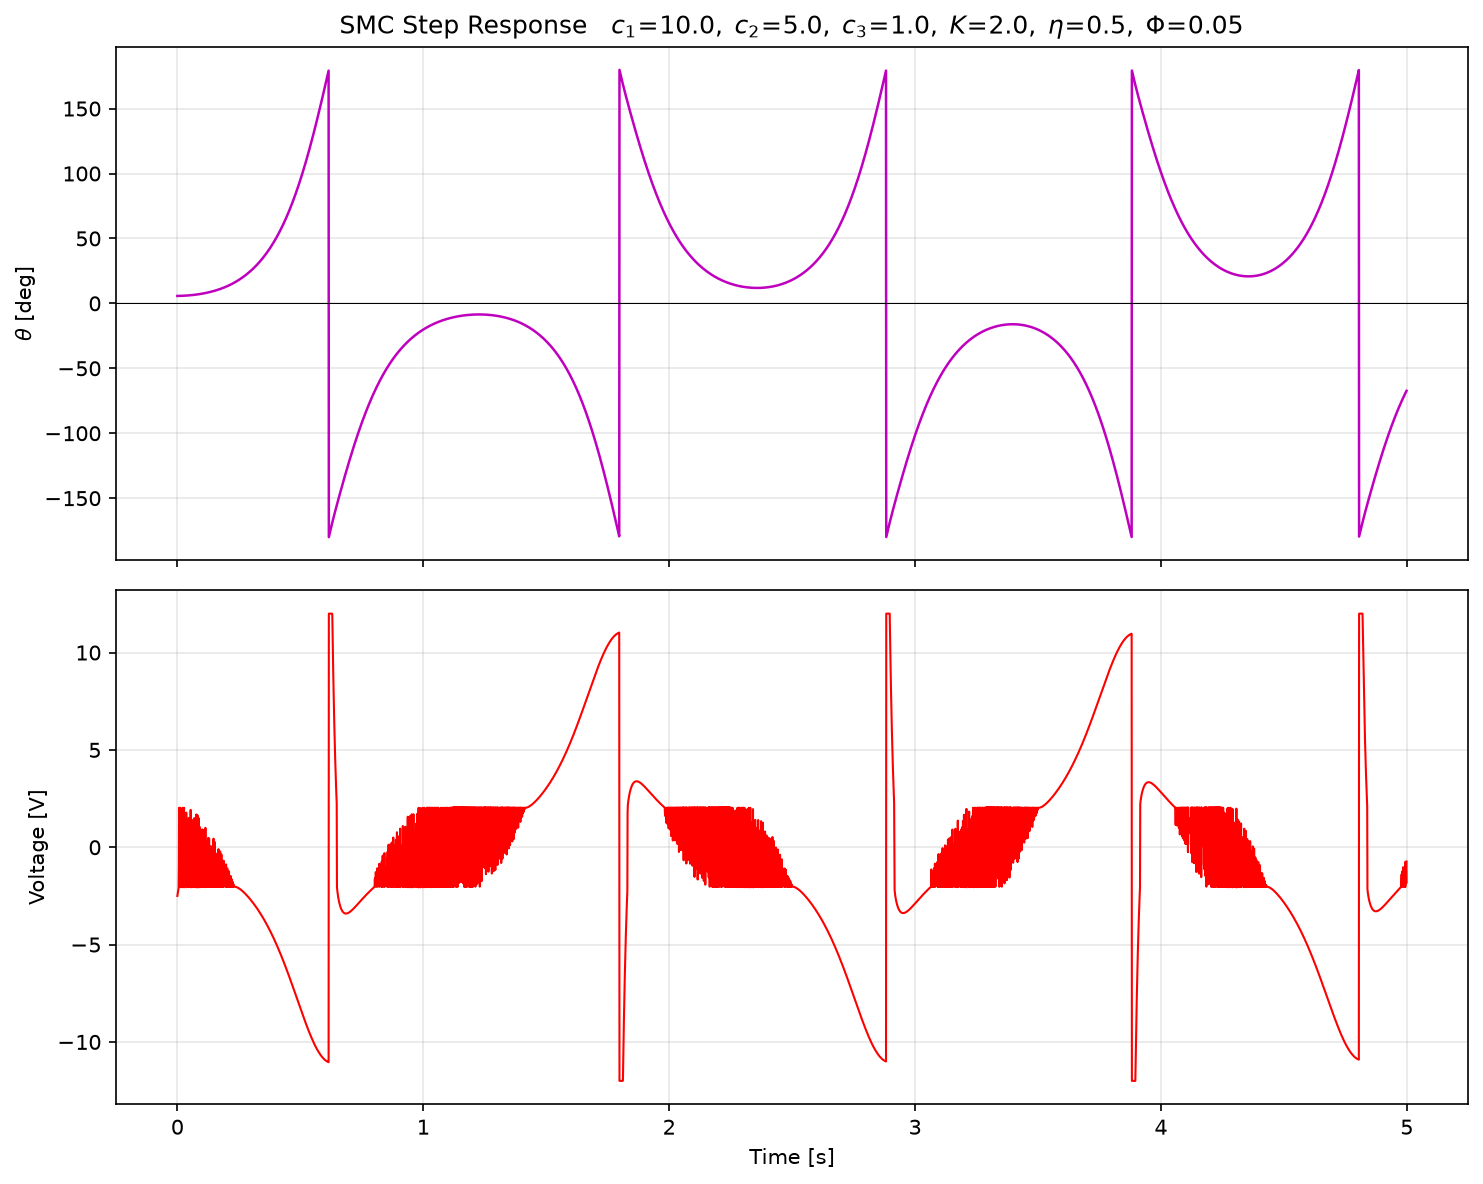
\includegraphics[width=0.85\textwidth]{results/smc_step_response.png}
\caption{پاسخ پله کنترلر مد لغزشی با لایه مرزی ($\theta_0 = 0.1$ رادیان)}
\label{fig:smc-step}
\end{figure}

% ─────────────────────────────────────────────────────────────────────
\subsection{مقایسه روش‌ها}

جدول زیر خلاصه‌ای از ویژگی‌های هر کنترلر را ارائه می‌دهد:

\begin{table}[H]
\centering
\caption{مقایسه روش‌های کنترل}
\begin{tabular}{llll}
\toprule
\textbf{کنترلر} & \textbf{حالت‌های استفاده‌شده} & \textbf{پارامترهای اصلی} & \textbf{خروجی} \\
\midrule
بدون کنترل & --- & --- & $V = 0$ \\
دستی & --- & $V_{\text{set}}$ & $V = V_{\text{set}}$ \\
PID & $\theta,\;\dot\theta$ & $K_p,\;K_i,\;K_d$ & $V = K_p\theta + K_i\!\int\theta + K_d\dot\theta$ \\
LQR & $\theta,\;\dot\theta,\;\dot\varphi,\;i_a$ & $\mathbf{Q},\;r$ & $V = -\mathbf{Kx}$ \\
مد لغزشی & $\theta,\;\dot\theta,\;\dot\varphi$ & $c_1,c_2,c_3,\;K,\;\eta,\;\Phi$ & $V = -K\,\text{sat}(s/\Phi) - \eta\,s$ \\
\bottomrule
\end{tabular}
\end{table}

شکل~\ref{fig:three-comparison} مقایسه هم‌زمان پاسخ پله سه کنترلر PID، LQR و مد لغزشی را نشان می‌دهد.

\begin{figure}[H]
\centering
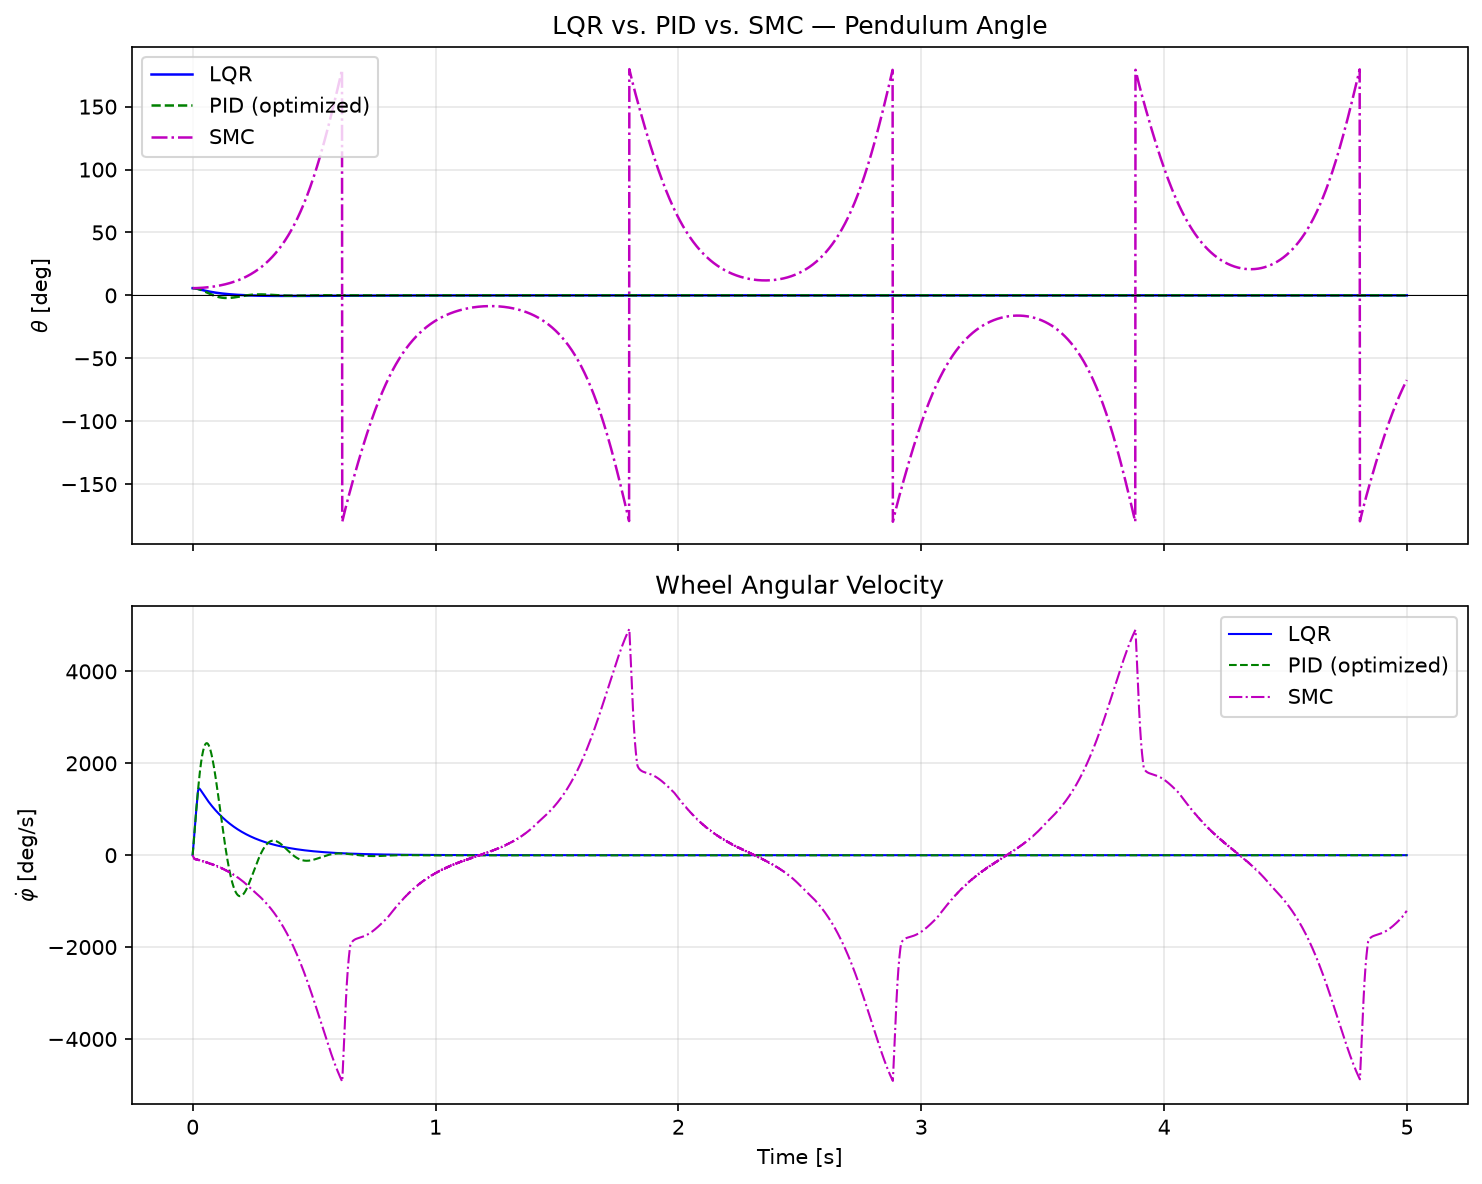
\includegraphics[width=0.85\textwidth]{results/three_controller_comparison.png}
\caption{مقایسه پاسخ پله کنترلرهای PID، LQR و مد لغزشی ($\theta_0 = 0.1$ رادیان)}
\label{fig:three-comparison}
\end{figure}

کنترلر LQR به دلیل استفاده از مدل کامل چهارحالته و بهینه‌سازی هم‌زمان، سریع‌ترین زمان نشست و کمترین نوسان را در میان سه روش دارد. کنترلر PID با ساختار ساده‌تر، پاسخ قابل‌قبولی ارائه می‌دهد، اما اندکی بیش‌جهت بیشتر و زمان نشست طولانی‌تری نسبت به LQR دارد. کنترلر مد لغزشی از نظر مقاومت در برابر عدم قطعیت پارامترها برتری دارد؛ هرچند به دلیل استفاده از لایه مرزی، همگرایی آن کمی هموارتر و با شیب ملایم‌تری نسبت به دو روش دیگر صورت می‌گیرد.

نکته مشترک تمامی روش‌ها این است که خروجی آن‌ها ولتاژ آرمیچر است. فیزیک موتور شامل نیروی ضد محرکه، سلف، مقاومت و نسبت تبدیل ($N=1$، اتصال مستقیم) به‌صورت داخلی در شبیه‌ساز رسیدگی می‌شود و کنترلرها هرگز مستقیماً گشتاور محاسبه نمی‌کنند.

از نظر عملکردی، کنترلر PID ساده‌ترین ساختار را دارد و برای سیستم‌هایی با دینامیک نسبتاً کند مناسب است. کنترلر LQR با استفاده از مدل کامل سیستم و بهینه‌سازی تابع هزینه، عملکرد بهتری در نزدیکی نقطه تعادل ارائه می‌دهد. کنترلر مد لغزشی در برابر عدم قطعیت پارامترها مقاوم‌تر است، اما طراحی آن نیازمند انتخاب دقیق ضخامت لایه مرزی برای مصالحه بین چترینگ و دقت است.

% ─────────────────────────────────────────────────────────────────────
\subsection{نتایج عددی تنظیم بهره}
\label{sec:gain-results}

در این بخش، نتایج عددی محاسبه بهره‌های بهینه برای کنترلرهای LQR و PID ارائه می‌شود. این مقادیر با استفاده از پارامترهای فیزیکی پیش‌فرض سیستم (جدول‌های بخش~\ref{sec:system-math}) و حل عددی معادله ریکاتی و بهینه‌سازی ITAE به‌دست آمده‌اند.

\subsubsection{بهره‌های بهینه LQR}

با انتخاب ماتریس‌های وزن زیر:

\begin{equation}
\mathbf{Q} = \operatorname{diag}(100,\; 1,\; 10,\; 0.01), \qquad r = 1.0
\end{equation}

حل معادله جبری ریکاتی با ماتریس‌های به‌روز‌شده ($N=1$)، بردار بهره بهینه زیر را تولید می‌کند:

\begin{equation}
\mathbf{K} = \begin{bmatrix} -844.46 & -138.69 & -2.32 & 0.16 \end{bmatrix}
\end{equation}

قطب‌های حلقه‌بسته سیستم با این بهره‌ها عبارتند از:

\begin{equation}
\lambda_1 \approx -2374.6, \quad \lambda_2 \approx -341.2, \quad \lambda_3 \approx -6.12, \quad \lambda_4 \approx -6.02
\end{equation}

دو قطب سریع ($\lambda_1$ و $\lambda_2$) مربوط به دینامیک الکتریکی آرمیچر هستند و دو قطب کندتر ($\lambda_3$ و $\lambda_4$) دینامیک مکانیکی پاندول را کنترل می‌کنند. قرارگیری تمام قطب‌ها در نیم‌صفحه چپ، پایداری مجانبی حلقه‌بسته را تضمین می‌کند.

شکل~\ref{fig:lqr-step} پاسخ پله کنترلر LQR را با این بهره‌ها نشان می‌دهد.

\begin{figure}[H]
\centering
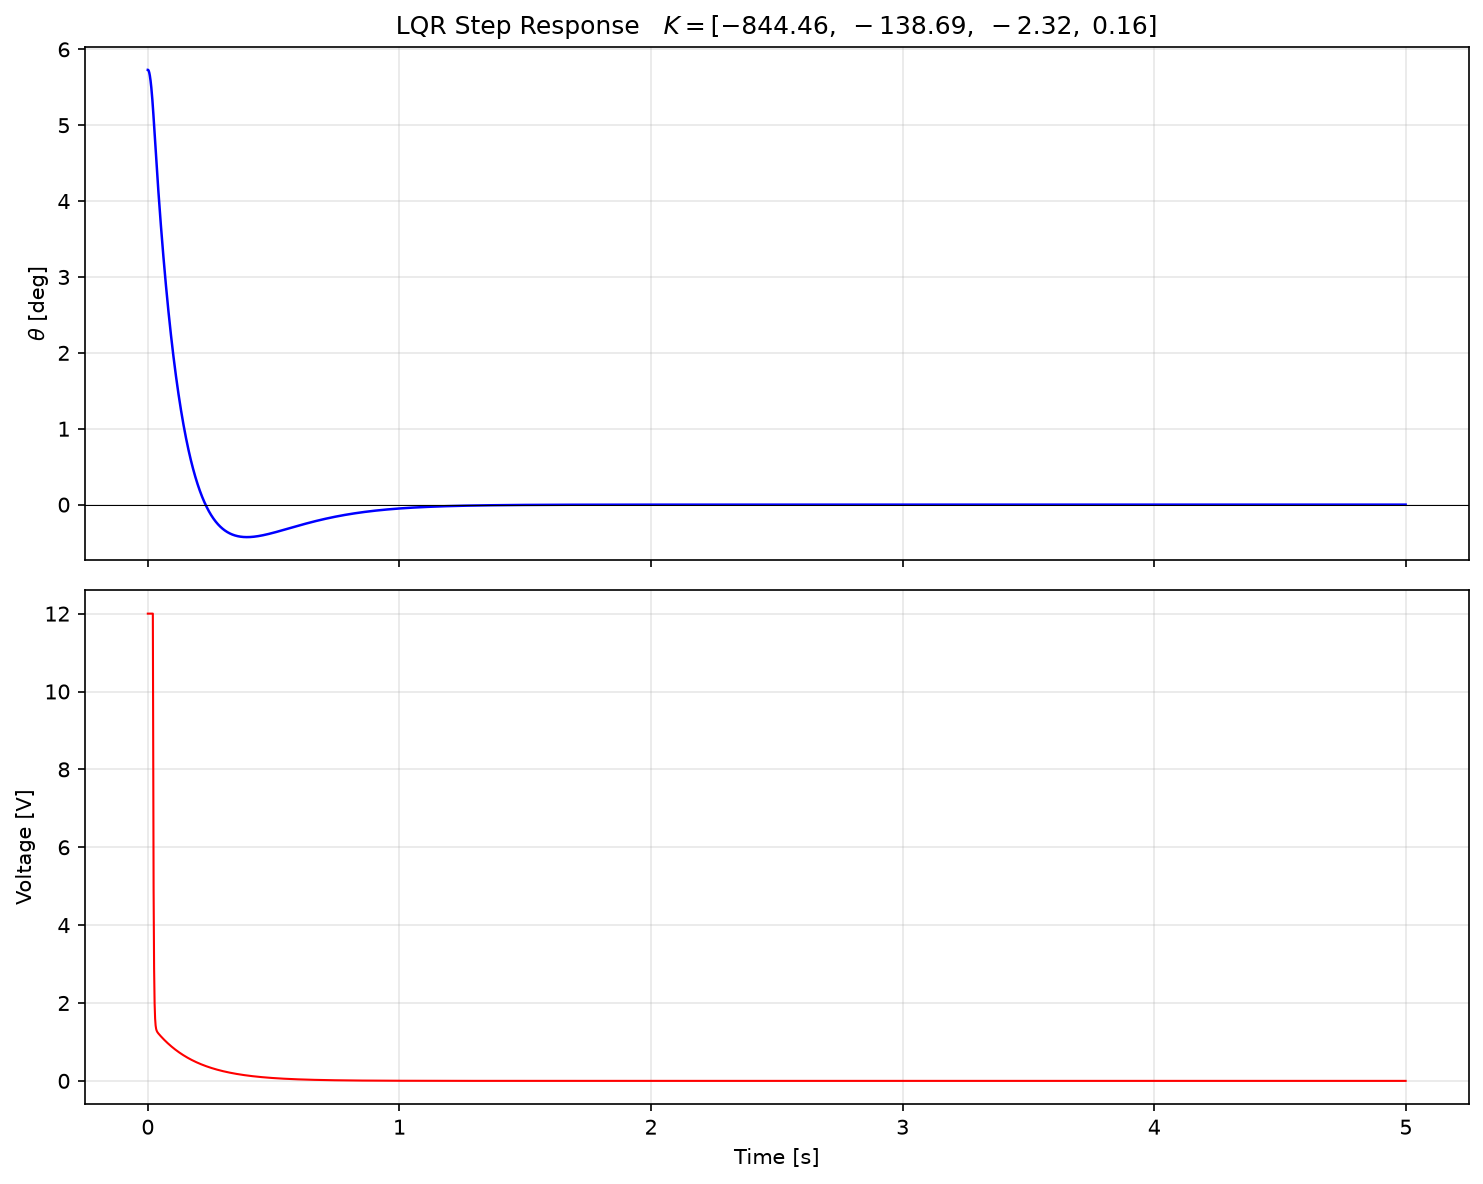
\includegraphics[width=0.85\textwidth]{results/lqr_step_response.png}
\caption{پاسخ پله کنترلر LQR با بهره‌های بهینه ($\theta_0 = 0.1$ رادیان)}
\label{fig:lqr-step}
\end{figure}

\subsubsection{بهره‌های بهینه PID}

بهره‌های PID با کمینه‌سازی شاخص عملکرد ITAE (انتگرال زمان ضربدر قدر مطلق خطا) و با استفاده از الگوریتم بهینه‌سازی نلدر--مید به‌دست آمده‌اند. شرایط شبیه‌سازی: زاویه اولیه $\theta_0 = 0.1$ رادیان، افق زمانی $T = 5$ ثانیه و گام زمانی $\Delta t = 0.001$ ثانیه.

\begin{equation}
K_p = 23.21, \qquad K_i = 0.208, \qquad K_d = 5.55
\end{equation}

مقدار بهینه شاخص ITAE برابر $2.280$ است. بهره مشتقی بزرگ‌تر از بهره تناسبی نیست، اما نقش قابل‌توجهی در میرایی نوسانات ایفا می‌کند. بهره انتگرالی کوچک ولی غیرصفر، خطای ماندگار ناشی از اغتشاش‌های ثابت را جبران می‌نماید.

شکل~\ref{fig:pid-step} پاسخ پله کنترلر PID را با این بهره‌ها نشان می‌دهد.

\begin{figure}[H]
\centering
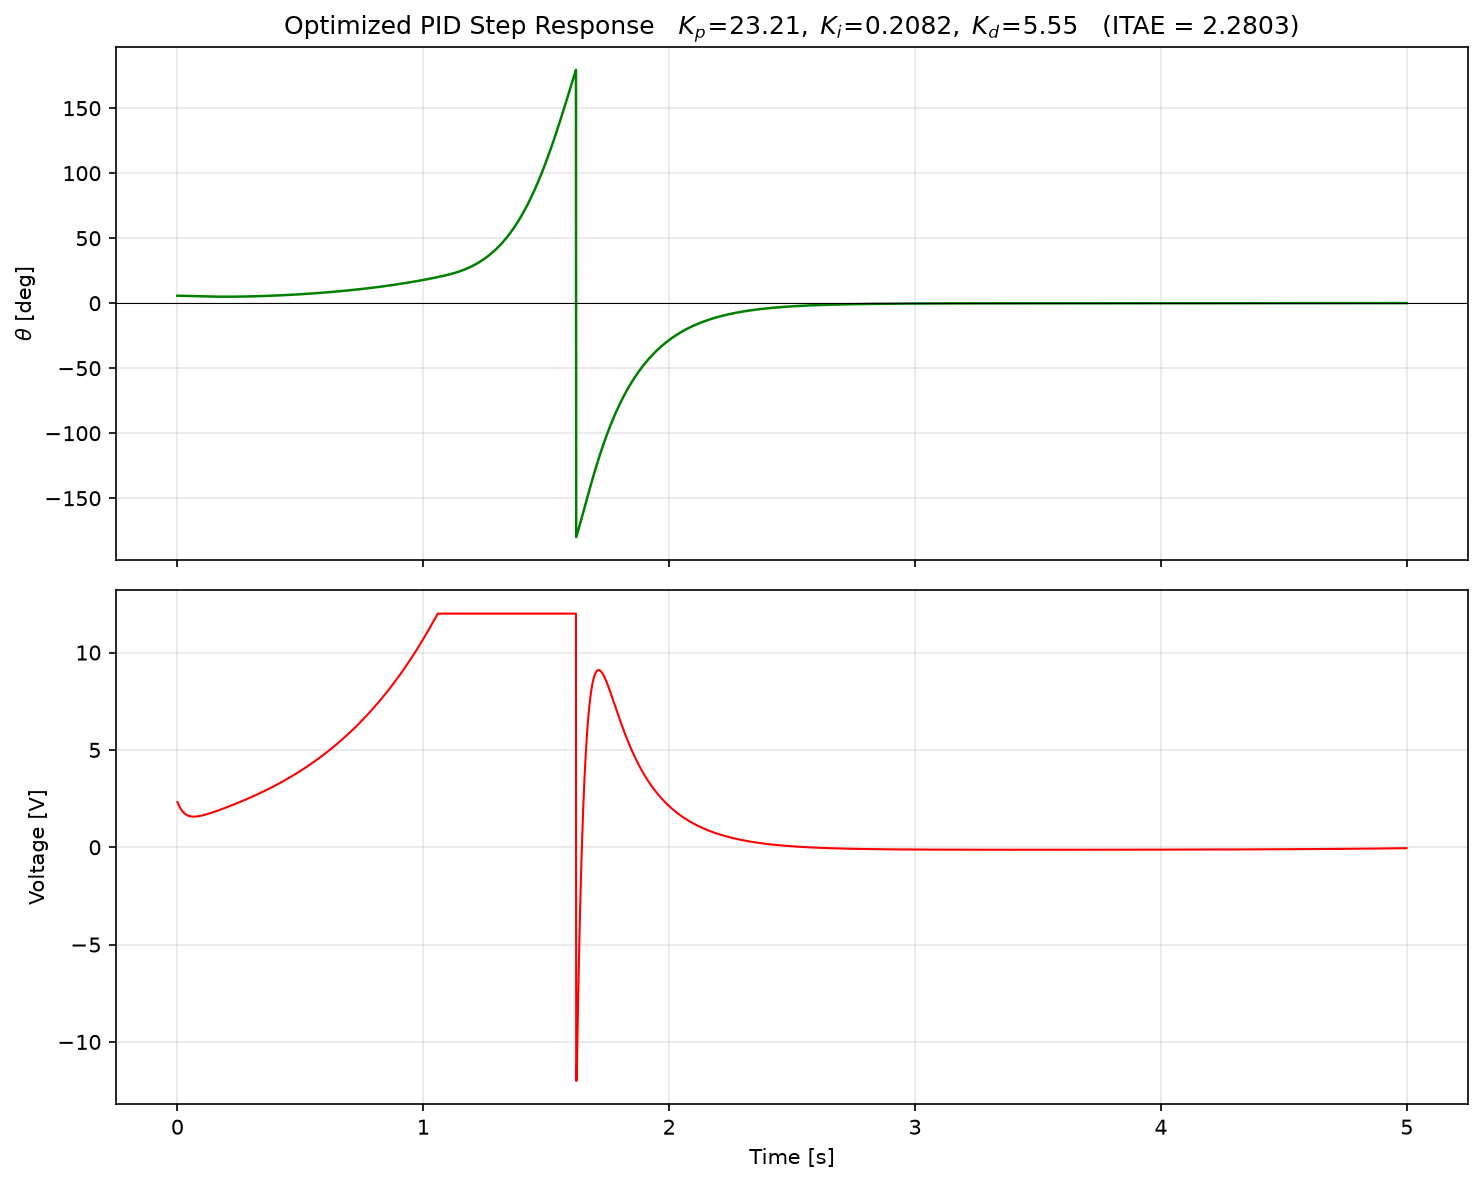
\includegraphics[width=0.85\textwidth]{results/pid_step_response.png}
\caption{پاسخ پله کنترلر PID با بهره‌های بهینه ITAE ($\theta_0 = 0.1$ رادیان)}
\label{fig:pid-step}
\end{figure}

\subsubsection{مقایسه عملکرد LQR و PID}

شکل~\ref{fig:lqr-vs-pid} مقایسه مستقیم پاسخ پله دو کنترلر را نشان می‌دهد. کنترلر LQR به دلیل استفاده از مدل کامل چهارحالته (شامل دینامیک الکتریکی) و بهینه‌سازی هم‌زمان تمام حالت‌ها، سرعت همگرایی بالاتر و نوسان کمتری نسبت به PID دارد. در مقابل، PID با ساختار ساده‌تر و تنها سه پارامتر تنظیم، پیاده‌سازی و درک شهودی آسان‌تری ارائه می‌دهد.

\begin{figure}[H]
\centering
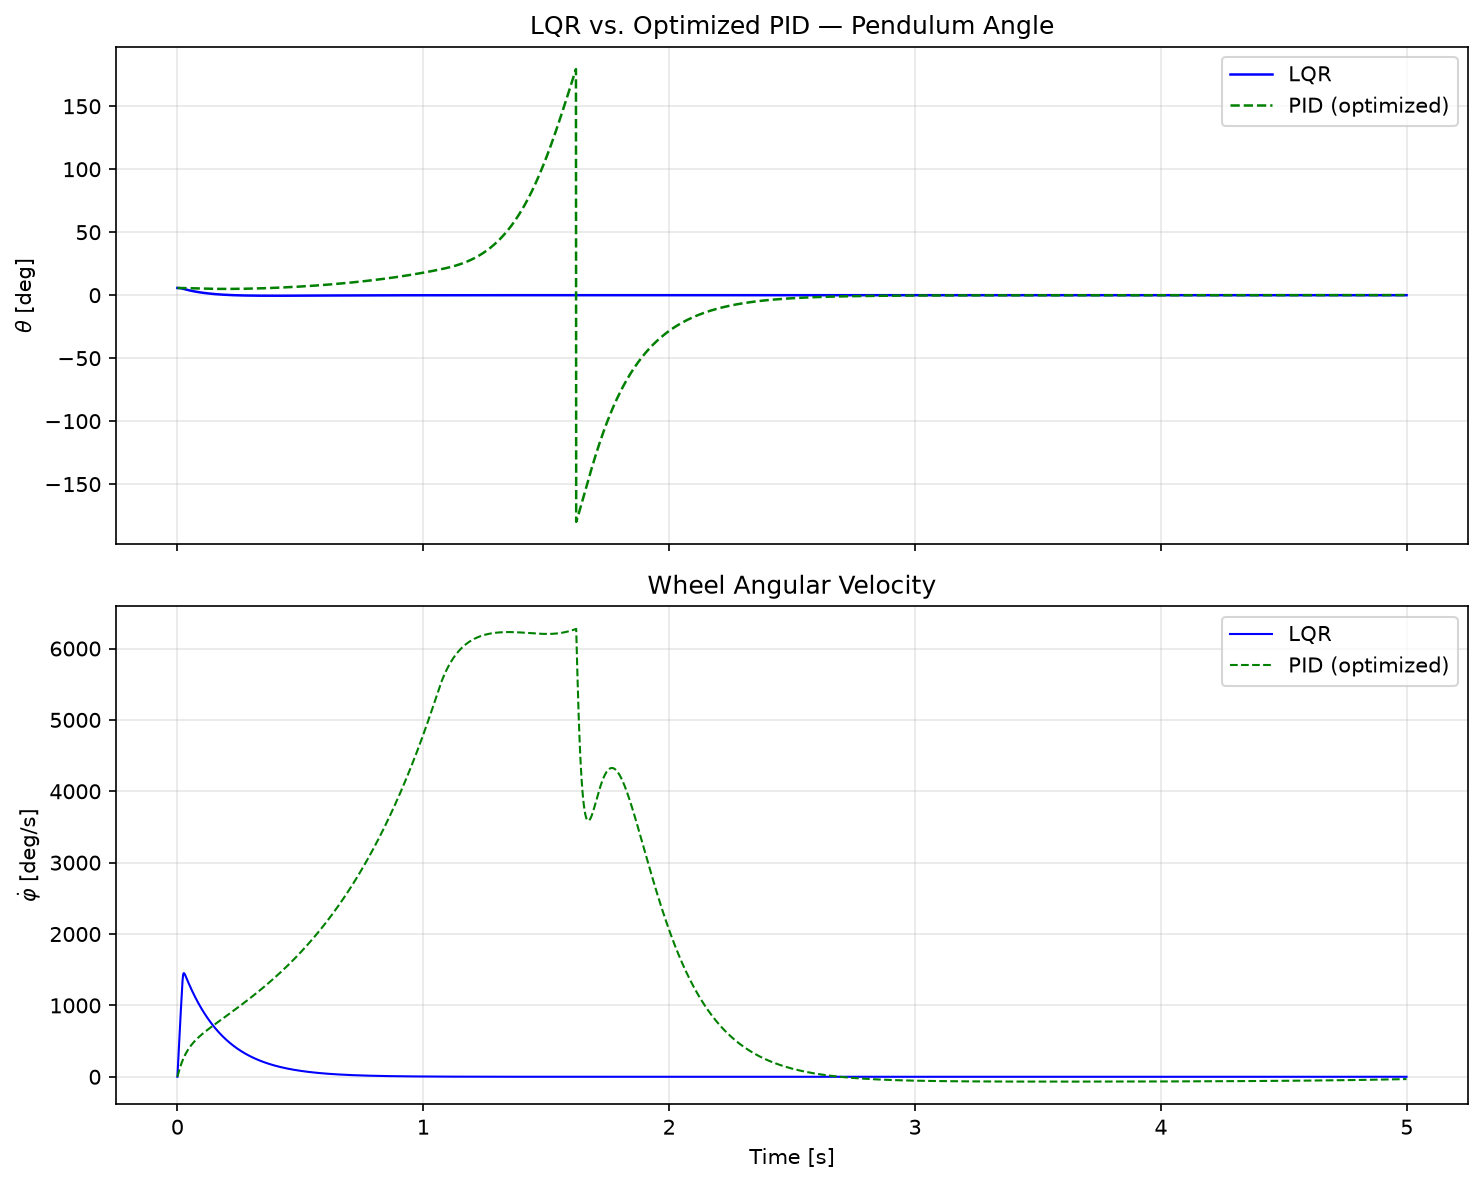
\includegraphics[width=0.85\textwidth]{results/lqr_vs_pid_comparison.png}
\caption{مقایسه پاسخ پله کنترلرهای LQR و PID ($\theta_0 = 0.1$ رادیان)}
\label{fig:lqr-vs-pid}
\end{figure}

جدول~\ref{tab:gain-summary} خلاصه‌ای از بهره‌های بهینه هر دو کنترلر را ارائه می‌دهد.

\begin{table}[H]
\centering
\caption{خلاصه بهره‌های بهینه محاسبه‌شده}
\label{tab:gain-summary}
\begin{tabular}{lll}
\toprule
\textbf{کنترلر} & \textbf{بهره‌ها} & \textbf{شاخص عملکرد} \\
\midrule
LQR & $K = [-844.46,\; -138.69,\; -2.32,\; 0.16]$ & قطب‌ها: $\approx -2374.6,\; -341.2,\; -6.12,\; -6.02$ \\
PID & $K_p = 23.21,\; K_i = 0.208,\; K_d = 5.55$ & $\text{ITAE} = 2.280$ \\
\bottomrule
\end{tabular}
\end{table}

\subsubsection{پارامترهای عددی کنترلر مد لغزشی}

پارامترهای پیش‌فرض کنترلر مد لغزشی استفاده‌شده در شبیه‌سازی‌ها به صورت زیر است:

\begin{equation}
c_1 = 10.0, \qquad c_2 = 5.0, \qquad c_3 = 1.0, \qquad K = 2.0, \qquad \eta = 0.5, \qquad \Phi = 0.05
\end{equation}

با این پارامترها، سطح لغزشی $s = 10\,\theta + 5\,\dot{\theta} + \dot{\varphi}$ تعریف می‌شود. نتایج شبیه‌سازی نشان می‌دهند که متغیر $s$ در چند صد میلی‌ثانیه نخست به لایه مرزی $|s| \le \Phi$ وارد شده و پس از آن، حرکت سیستم بر روی منیفولد لغزشی با همگرایی هموار به سمت تعادل ادامه می‌یابد. ضخامت لایه مرزی $\Phi = 0.05$ رادیان، مصالحه مناسبی بین کاهش چترینگ و حفظ دقت ردیابی ایجاد می‌کند.